\chapter{质点动力学（下）}
\setcounter{example_counter}{1}

\section{动量守恒}

\vspace{-0.3em}

\subsection{动量定理}

\vspace{-0.3em}

\subsubsection{质点的动量定理}

\vspace{-0.3em}

质点的动量$\vec{p}=m\vec{v}$，力$\vec{F}$对质点的冲量为$\vec{I}=\displaystyle\int_{t_1}^{t_2}\vec{F}dt$. 特别地，恒力的冲量$\vec{I}=\vec{F}\Delta t$.

质点所受合外力的冲量等于其动量的变化。

\begin{formula}
    $d\vec{I}=\vec{F}dt=d\vec{p},~~\vec{I}=\displaystyle\int_{t_1}^{t_2}\vec{F}dt=\Delta \vec{p}$
\end{formula}

%\note{质点的动量定理，其实就是牛顿第二定律的变形。}

\subsubsection{质点系的动量定理}

对于多个质点组成的系统，合外力的冲量等于动量的变化，与内力无关。

\begin{formula}
    $\vec{I}_{\text{外}}=\Delta \vec{P}$
\end{formula}

\begin{example}{质点的动量定理}
    粗糙水平面上放一个质量为$\SI{1}{kg}$的物体，静摩擦因数$\mu_s=0.20$，滑动摩擦因数$\mu=0.16$，现用一水平力推该物体，大小$F=t+1$(SI)，$g=\SI{10}{m/s^2}$. 求：(1) 物体所受合外力与$t$的关系；(2) 第$\SI{2}{s}$末的速度；(3) 前两秒内的位移；(4) $F$在前两秒内做的功。

    \tcblower

    (1)~最大静摩擦力$f_m=\mu_s mg=\SI{2}{N}$，当$F=t+1\leq \SI{2}{N}$，即$t\leq \SI{1}{s}$时，推不动物体，合力为零。

    而当$t>\SI{1}{s}$时，已超过静摩擦力，能推动物体，所受合外力为$F-\mu mg=t+1-1.6=t-0.6$(SI)

    \vspace{0.3em}

    (2)~力$F$在$t~(t>1)$时间前的冲量为$\displaystyle\int_1^t{(t-0.6)dt}=\left.\left(\dfrac{1}{2}t^2-0.6t\right)\right|_1^t=0.5t^2-0.6t+0.1$

    \vspace{0.3em}
    
    利用动量定理，可得$0.5t^2-0.6t+0.1=mv$，求得$v=0.5t^2-0.6t+0.1$，代入$t=2$得$v=\SI{0.9}{m/s}$

    \vspace{0.3em}

    (3)~对$v$进行积分可得位移，$x=\displaystyle\int_1^2{(0.5t^2-0.6t+0.1)dt}=\left.\left(\dfrac{1}{6}t^3-0.3t^2+0.1t\right)\right|_1^2=\dfrac{11}{30}~\unit{m}$

    \vspace{0.3em}

    (4)~利用动能定理，$W-\mu mgx=\dfrac{1}{2}mv^2$，得$W=\dfrac{119}{120}\unit{J}$
    
    \tcbline

    %【补充练习】质量为$m$的小球被轻绳挂在天花板上，做圆锥摆运动，角速度为$\omega$. 求转动一周过程中，重力和绳子的拉力对小球的冲量大小。
    
    \begin{minipage}{0.83\textwidth}
    \setlength{\parskip}{0.5em}
    \linespread{1.3}

    【补充练习】质量为$m$的小球被轻绳挂在天花板上，做圆锥摆运动，角速度为$\omega$. 求转动一周过程中，重力和绳子的拉力对小球的冲量大小。
    \end{minipage}
    \hfill
    \begin{minipage}{0.12\textwidth}
        \vspace{-0.5em}
        \centering 
\includegraphics[width=\textwidth]{asset/ch3/T1.png}
    \end{minipage}
    

\end{example}

\begin{example}{连续体的动量定理}
    水平放置的均匀水管弯曲成$90^\circ$，水流量为$\SI{3}{kg/s}$，流速为$\SI{10}{m/s}$，求水流在转角处对弯管的压力大小。（水的密度$\rho=\SI{1e3}{kg/m^3}$）
    \tcblower

    \begin{minipage}{0.82\textwidth}
    \linespread{1.5}
    \setlength{\parskip}{0.1em}
    设水管横截面积为$S$，选择包含弯折部分在内的一段液体作为研究对象。
    
    在$dt$的时间内，发生变化的部分的水的质量$m=Qdt$
    
    它的初末速度可记为$\vec{v}_1=-v\hat{j},~\vec{v}_2=v\hat{i}$

    根据动量定理，$\vec{F}dt=m(\vec{v}_2-\vec{v}_1)$，代入数据得$\vec{F}=\SI{30}(\hat{i}+\hat{j})$
    
    \end{minipage}
    \hfill
    \begin{minipage}{0.15\textwidth}
        \centering 
\includegraphics[width=\textwidth]{asset/ch3/T2.png}
    \end{minipage}

    \vspace{0.3em}

    这说明水管对水的压力大小为$30\sqrt{2}~\unit{N}$，根据牛顿第三定律，水对水管的压力大小也为此值。

    \tcbline

    \begin{minipage}{0.73\textwidth}
    【补充练习】装煤车以$v=\SI{3}{m/s}$的速率在煤斗下方通过，每秒钟落入车厢的煤是$\Delta m=\SI{500}{kg}$，若要使车厢速率不变，忽略摩擦，要用多大的牵引力拉车厢？
    \end{minipage}
    \hfill
    \begin{minipage}{0.25\textwidth}
        \centering 
\includegraphics[width=\textwidth]{asset/ch3/T4.png}
    \end{minipage}
    
\end{example}

\subsection{动量守恒定律}

\subsubsection{动量守恒的条件}

若质点系所受合外力为零，质点系的总动量不变。质点系的内力对总动量不产生影响。

\begin{formula}
    若$\vec{F}_{\text{外}}=\vec{0}$，则$\vec{P}=\mathrm{const.}$
\end{formula}

\begin{example}{动量守恒定律}

    \begin{minipage}{0.78\textwidth}
    质量为$m_A=\SI{2}{kg},~m_B=\SI{3}{kg}$的长方形物体A、B并排放在光滑桌面上，现有质量为$m=\SI{100}{g}$的子弹以速率$v_0=\SI{800}{m/s}$水平射入物体A，经$\SI{0.01}{s}$进入物体B，最后留在物体B内部。若子弹射入A的过程中，所受摩擦力恒
    \end{minipage}
    \hfill
    \begin{minipage}{0.2\textwidth}
        \centering 
\includegraphics[width=\textwidth]{asset/ch3/T3.png}
    \end{minipage}

    \vspace{0.5em}

    为$\SI{3e3}{N}$，求：(1)~子弹射入A的过程中，A对B的作用力大小；(2)~最后A、B的速度大小。

    \tcbline
    
    \setlength{\parskip}{0.1em}

    (1)~在子弹射入A的过程中，A和B是一起运动的，将A、B视为一个整体，$f=(m_A+m_B)a$

    而采用隔离法，只分析B物体，可得$F_{AB}=ma$，代入数据可得$F_{AB}=\SI{1.8e3}{N}$

    (2)~在子弹射入A的过程中，对A、B构成的系统，$ft=(m_A+m_B)v_A$，得$v_A=\SI{6}{m/s}$

    在子弹射入B之后，A与B脱离，A就保持这个速度，而子弹会和B一起继续加速到$v_B$

    对所有物体构成的系统，在整个过程中动量守恒，$mv_0=m_Av_A+(m_B+m)v_B$，解得$v_B\approx \SI{21.9}{m/s}$

    \tcblower
    \setlength{\parskip}{0.1em}
    【补充练习】判断下列说法是否正确：
    
    (1)~作用力与反作用力的冲量之和一定为零；(2)~系统的内力不改变系统的总动量；
    
    (3)~合外力冲量的方向与系统总动量的变化相同；(4)~恒力作用于质点，则时间越长，质点动量越大。
\end{example}

\subsubsection{碰撞}

在碰撞、爆炸等问题中，因为力的作用时间极短，可近似认为动量守恒。

\begin{example}{碰撞}
    在一次粒子散射实验中，质量为$m$的粒子A撞向质量为$M$的静止粒子B。碰撞后A、B的运动方向与A原运动方向的夹角分别为$60^\circ, 30^\circ$，求A粒子碰撞后与碰撞前的速率之比。

    \tcblower

    \begin{minipage}{0.75\textwidth}
    以A原运动方向为$x$正方向
    
    设A粒子碰撞前速率为$v_0$，碰撞后两粒子速率为$v_A,v_B$

    \vspace{0.5em}
        
    根据$y$方向动量守恒，$0=\dfrac{\sqrt{3}}{2}mv_A+\dfrac{1}{2}Mv_B$，即$Mv_B=\sqrt{3}mv_A$

    \vspace{0.5em}

    根据$x$方向动量守恒，$mv_0=\dfrac{1}{2}mv_A+\dfrac{\sqrt{3}}{2}Mv_B$，代入可解得$\dfrac{v_A}{v_0}=\dfrac{1}{2}$
  
    \end{minipage}
    \hfill
    \begin{minipage}{0.22\textwidth}
        \centering 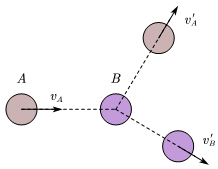
\includegraphics[width=\textwidth]{asset/ch3/T21.png}
    \end{minipage}

    
    
    \tcbline
    【补充练习】
    小球A的质量是B的$4$倍，二者发生碰撞。碰撞前$\vec{v}_A=3\hat{i}+4\hat{j},~\vec{v}_B=2\hat{i}-7\hat{j}$，分别在以下情况下求碰撞后速度: (1) 碰撞后$\vec{v}_B^\prime=7\hat{i}-4\hat{j}$；(2) 碰撞后粘在一起。
\end{example}


\subsubsection{人船模型}

人船模型也可以视为“类碰撞”的情形，在水平方向动量守恒。

%人船模型也可以视为“类碰撞”的情形，水平方向动量守恒，有两种解题思路：
%\begin{itemize}
%    \item 可利用任意时刻的动量为零，得到速度关系，再积分得到位移关系
%    \item 直接利用质心运动定理，质心的水平坐标不变，直接得到位移关系
%\end{itemize}

\begin{example}{人船模型}
    带有1/4圆弧光滑圆槽的大物体质量为$M$，停在光滑的水平面上，滑槽半径为$R$，质量为$m$的小物体自顶点下滑，求小物体滑到底时，大物体在水平面上移动的距离，大物体相对于地面的速度。
    
    \tcblower

    \begin{minipage}{0.7\textwidth}
    (1)~两物体构成的系统在水平方向不受外力，动量守恒
    
    在任意时刻，$0=-MV+mv_x$

    \vspace{0.3em}

    两边同时积分，可得$M\displaystyle\int{Vdt}=m\int{v_xdt}$，即$MS=ms$

    \vspace{0.5em}

    结合几何关系，$S+s=R$，可得$S=\dfrac{m}{M+m}R$

    %\vspace{0.3em}

    %{\fangsong 注：本题也可采用质心运动定理进行求解。
    
    %因为水平方向不受外力，所以质心的横坐标不会变化。

    %\vspace{0.5em}

    %根据$0=\dfrac{-MS+m(R-S)}{M+m}$，也可解得$S=\dfrac{m}{M+m}R$}

    \vspace{0.5em}
    
    (2)~小物体滑到底端时，小物体速度为水平方向
    
    根据动量守恒定律，仍有$0=-MV+mv$

    \vspace{0.5em}

    根据机械能守恒定律，$mgR=\dfrac{1}{2}MV^2+\dfrac{1}{2}mv^2$

    \vspace{0.5em}

    联立两式解得$V=\sqrt{\dfrac{2m^2gR}{M(M+m)}}$
  
    \end{minipage}
    \hfill
    \begin{minipage}{0.27\textwidth}
        \centering 
\includegraphics[width=\textwidth]{asset/ch3/T5.png}
    \end{minipage}

    \tcbline
    
    \begin{minipage}{0.78\textwidth}
    【补充练习】质量为$m$的小物体从质量为$M$、倾角为$\theta$、长为$L$的斜面顶端静止滑落，不计摩擦，求小物体滑落到斜面底端时，斜面的位移和速度。
    \end{minipage}
    \hfill
    \begin{minipage}{0.2\textwidth}
        \centering 
\includegraphics[width=\textwidth]{asset/ch3/T6.png}
    \end{minipage}
       
\end{example}

\section{角动量守恒}

\subsection{角动量定理}

\subsubsection{力矩}

对固定点O而言，若质点的位置矢量为$\vec{r}$，则力$\vec{F}$的力矩定义为$\vec{M}=\vec{r}\times \vec{F}$

力矩的大小其实就是杠杆原理中的力乘以力臂，方向可简化区分顺时针/逆时针转动。

\note{如果力过固定点O，则力臂为零，力矩就为零，因为对于转动无作用。}

\subsubsection{角动量}

对固定点O而言，质点的角动量定义为$\vec{L}=\vec{r}\times \vec{p}=\vec{r}\times (m\vec{v})$

角动量的大小与力矩计算方法类似，等于动量乘以动量臂，方向也可简化区分顺时针/逆时针转动。

\note{特别地，对于圆周运动而言，对圆心的动量臂等于半径$R$，所以角动量的大小就等于$mvR$。}

\begin{figure}[htb]
    \centering
    
\includegraphics[width=0.45\linewidth]{asset/ch3/T7.png} 
\includegraphics[width=0.45\linewidth]{asset/ch3/T8.png}
\end{figure}

\begin{formula}
    $\text{力矩}M\text{的大小}=\text{力}F\times \text{力臂}$，$\text{角动量}L\text{的大小}=\text{动量}mv\times \text{动量臂}$
\end{formula}

\subsubsection{角动量定理}

对一个固定点O，合外力矩等于角动量的变化率。
\begin{formula}
    $\vec{M}=\dfrac{d\vec{L}}{dt},~~\displaystyle\int_0^t{\vec{M}dt}=\Delta \vec{L}$
\end{formula}

\subsection{角动量守恒定律}

对一个固定点O，若合外力矩为零，则系统的角动量守恒。

\warn{角动量守恒必须选定固定点O，对不同的点，角动量守恒的判断结果不同。}

\begin{formula}
    若$\vec{M}=\vec{0}$，则$\vec{L}=\mathrm{const.}$
\end{formula}

\note{如果系统不受外力，或外力过所选择的固定点，则合外力矩为零，就能满足角动量守恒的要求。例如，行星运动过程中，相对于中心天体的角动量守恒。}

\note{但是系统所受合外力是零，并不能说明合力矩也是零，因为两个力可能不共线，角动量不一定守恒。}

\begin{example}{角动量守恒定律}
    人造卫星绕地球沿椭圆轨道运动，地球半径为$R$，卫星到地面的最近、最远距离为$h_1,h_2$，(1)~若已知近地点速率为$v_1$，求远地点速率；(2)~若已知地球质量为$M$，求近地点和远地点速率。
    \tcblower

    (1)~根据角动量守恒定律，$mv_1(R+h_1)=mv_2(R+h_2)$，可得$v_2=v_1\dfrac{R+h_1}{R+h_2}$

    \vspace{0.5em}

    (2)~根据机械能守恒定律，$\dfrac{1}{2}mv_1^2+\left(-\dfrac{GMm}{R+h_1}\right)=\dfrac{1}{2}mv_2^2+\left(-\dfrac{GMm}{R+h_2}\right)$

    \vspace{0.5em}

    {\fangsong 注：此处不能用重力势能，而要用万有引力势能，注意万有引力势能的表达式自带负号。}

    结合角动量守恒定律$mv_1(R+h_1)=mv_2(R+h_2)$

    \vspace{0.5em}
    
    可联立解得$v_1=\sqrt{\dfrac{2GM(R+h_2)}{(R+h_1)(2R+h_1+h_2)}},~v_2=\sqrt{\dfrac{2GM(R+h_1)}{(R+h_2)(2R+h_1+h_2)}}$
   
    \tcbline

    \begin{minipage}{0.73\textwidth}
    【补充练习】质量为$m$的小球系于轻绳一端，另一端穿过桌面上的小孔并用手拉住。先使小球做半径为$r_0$的圆周运动，角速度为$\omega_0$；若拉动轻绳，使运动半径变为$r$。求：此时的角速度和拉力，拉力在这一过程中所做的功。
    \end{minipage}
    \hfill
    \begin{minipage}{0.25\textwidth}
        \centering 
\includegraphics[width=\textwidth]{asset/ch3/T9.png}
    \end{minipage}

\end{example}

\subsection{三大守恒的对比}

\begin{table}[htb]
    \centering
    \begin{tabular}{|c|c|c|}
        \hline
        守恒定律 & 条件 & 是否与内力有关\\
         \hline
        动量守恒 & 合外力为零 & 无关 \\
         \hline
        角动量守恒 & 合外力矩为零 & 无关 \\
         \hline
        机械能守恒 & 只有保守内力做功 & 有关 \\
         \hline
    \end{tabular}
\end{table}

\note{三大守恒分别对应了三种不同的对称性，彼此是相互独立的，任何一个物理量守恒，都不能直接推出其他的守恒结论。但单个质点的动量守恒，则角动量一定守恒。}

\begin{example}{三大守恒的对比}
    \setlength{\parskip}{0.1em}
    判断在以下情境中，动量、机械能、对圆心的角动量是否守恒。

    (1)~竖直平面内由绳牵引的圆周运动；(2)~竖直平面内由杆控制的匀速圆周运动

    \tcblower

    \setlength{\parskip}{0.1em}

    判断是否守恒可以从条件上判断，也可以从结果上判断。

    (1)~只有重力做功，机械能守恒；速度的大小和方向时刻变化，所以动量、角动量不守恒。

    (2)~速度大小不变，半径不变，所以角动量守恒；速度方向改变，所以动量不守恒；动能不变，势能改变，机械能不守恒。
    
    \tcbline

    \setlength{\parskip}{0.1em}
    
    【补充练习】一质点在几个外力同时作用下运动时，判断下列叙述是否正确。
    
    (1)~若质点的动量改变，动能一定改变；(2)~若动量守恒，则机械能守恒；

    (3)~若动量守恒，则对任意点的角动量守恒；(4)~若外力做功为零，外力的冲量一定为零；
    
    (5)~若机械能守恒，则动量守恒；(6)~若对一点的角动量守恒，则对其他任意点的角动量也守恒

\end{example}

\section{拓展内容}

\subsection{变质量系统的动量守恒}

如果系统质量发生变化，则不能贸然使用牛顿第二定律，动量的变化需要同时考虑质量和速度的变化。

使用数学上的全微分，可知

\begin{formula}
    $d\vec{p}=m\cdot d\vec{v}+\vec{v}\cdot dm$
\end{formula}

\begin{example}{变质量系统的动量守恒*}
    (1) 质量为$M$的火箭以速度$v$运动，以相对速率$u$向后扔出一个质量为$m$的球，求火箭的速度。

    (2) 质量为$M$的火箭以速度$v$运动，以相对速率$u$持续向后喷出气体，求质量减小$m$时的速度。

    \tcblower
    
    (1)~飞船的初动量为$Mv$，且动量守恒，$Mv=(M-m)v^\prime+m(v^\prime-u)$，解得$v^\prime=v+\dfrac{m}{M}u$

    (2)~在$dt$时间内，假设喷出气体质量为$dm$，速度增加$dv$
    
    则飞船的动量变为$(M-dm)(v+dv)$，而喷出气体的动量为$dm(v+dv-u)$（注意速度方向）

    \vspace{0.25em}

    根据动量守恒定律，$Mv=(M-dm)(v+dv)+(v+dv-u)dm$，整理得$dv=\dfrac{u}{M}dm$

    \vspace{0.5em}

    结合$dm=-dM$，两边积分得$\displaystyle\int{dv}=-\int\dfrac{u}{M}dM$，即$v^\prime-v=u[\ln{M}-\ln{(M-m)}]$

    \vspace{0.5em}

    整理得$v^\prime=v+u\ln{\dfrac{M}{M-m}}$

    \tcbline
    【补充练习】均匀竖直链条长度为$l$，质量为$m$，下端刚触地，求自由下落$h$时对地面的作用力。
\end{example}